\documentclass[tikz,border=4pt]{standalone}
\usepackage{ctex}
\usepackage{amsmath,amssymb}
\usetikzlibrary{calc,arrows.meta,patterns}
\begin{document}
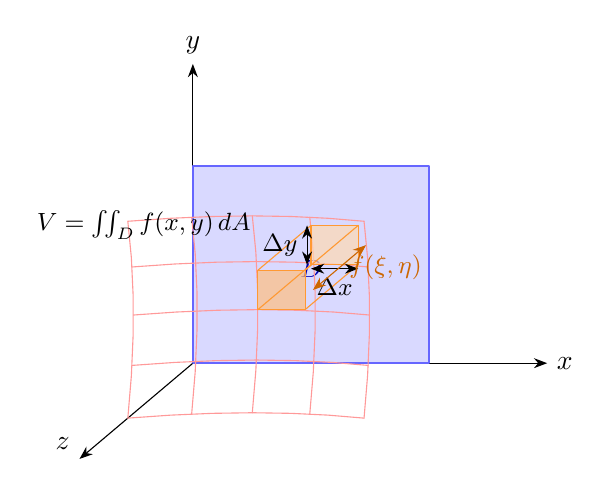
\begin{tikzpicture}[
  x={(1cm,0cm)}, y={(0cm,1cm)}, z={(-0.45cm,-0.38cm)},
  line cap=round, line join=round,
  >=Stealth
]
% 坐标轴
\draw[->] (0,0,0) -- (4.5,0,0) node[right] {$x$};
\draw[->] (0,0,0) -- (0,3.8,0) node[above] {$y$};
\draw[->] (0,0,0) -- (0,0,3.2) node[above left] {$z$};

% 积分区域 D（矩形 [0,3]x[0,2.5] 底面）
\fill[blue!15] (0,0,0) -- (3,0,0) -- (3,2.5,0) -- (0,2.5,0) -- cycle;
\draw[blue!60, thick] (0,0,0) -- (3,0,0) -- (3,2.5,0) -- (0,2.5,0) -- cycle;
\node[blue!70!black, font=\small] at (1.5,1.2,0) {$D$};

% 曲面 z = 1 + 0.1*(x-1.5)^2 + 0.15*(y-1.25)^2 的网格（简化）
\foreach \xi in {0,0.75,1.5,2.25,3} {
  \draw[red!40, thin]
    plot[domain=0:2.5, samples=6, variable=\yi]
      ({\xi},{\yi},{1.5+0.08*(\xi-1.5)*(\xi-1.5)+0.1*(\yi-1.25)*(\yi-1.25)});
}
\foreach \yi in {0,0.625,1.25,1.875,2.5} {
  \draw[red!40, thin]
    plot[domain=0:3, samples=7, variable=\xi]
      ({\xi},{\yi},{1.5+0.08*(\xi-1.5)*(\xi-1.5)+0.1*(\yi-1.25)*(\yi-1.25)});
}

% 小柱体（dV 示意）
\def\sx{1.5} \def\sy{1.25} \def\dx{0.6} \def\dy{0.5}
\def\zh{1.5} % z value at (sx,sy)
\fill[orange!30, opacity=0.7]
  (\sx,\sy,0) -- ({\sx+\dx},\sy,0) -- ({\sx+\dx},{\sy+\dy},0) -- (\sx,{\sy+\dy},0) -- cycle;
\fill[orange!50, opacity=0.7]
  (\sx,\sy,\zh) -- ({\sx+\dx},\sy,\zh) -- ({\sx+\dx},{\sy+\dy},\zh) -- (\sx,{\sy+\dy},\zh) -- cycle;
\draw[orange!80]
  (\sx,\sy,0) -- (\sx,\sy,\zh)
  ({\sx+\dx},\sy,0) -- ({\sx+\dx},\sy,\zh)
  ({\sx+\dx},{\sy+\dy},0) -- ({\sx+\dx},{\sy+\dy},\zh)
  (\sx,{\sy+\dy},0) -- (\sx,{\sy+\dy},\zh);
\draw[orange!80]
  (\sx,\sy,0) -- ({\sx+\dx},\sy,0) -- ({\sx+\dx},{\sy+\dy},0) -- (\sx,{\sy+\dy},0) -- cycle;
\draw[orange!80]
  (\sx,\sy,\zh) -- ({\sx+\dx},\sy,\zh) -- ({\sx+\dx},{\sy+\dy},\zh) -- (\sx,{\sy+\dy},\zh) -- cycle;

% 标注
\draw[<->] ({\sx-0.05},\sy,0) -- ({\sx-0.05},{\sy+\dy},0)
  node[midway, left, font=\small] {$\Delta y$};
\draw[<->] (\sx,{\sy-0.05},0) -- ({\sx+\dx},{\sy-0.05},0)
  node[midway, below, font=\small] {$\Delta x$};
\draw[<->, orange!80!black] ({\sx+\dx+0.1},{\sy+\dy/2},0) -- ({\sx+\dx+0.1},{\sy+\dy/2},\zh)
  node[midway, right, font=\small] {$f(\xi,\eta)$};

\node[font=\small, align=center] at (0.5,2.7,2.5)
  {$V = \iint_D f(x,y)\,dA$};
\end{tikzpicture}
\end{document}
